%%
%% Author: Maciej
%% 18.11.2018
%%

% Preamble
\documentclass[11pt]{article}
\usepackage{geometry}
 \geometry{
 a4paper,
 total={170mm,257mm},
 left=20mm,
 top=20mm,
 }

% Packages
\usepackage{amsmath}
\usepackage{pythontex}
\usepackage{graphicx}
\usepackage{caption}
\usepackage{float}
\restylefloat{table}
\usepackage{array}
\usepackage{makecell}

\renewcommand\theadalign{bc}
\renewcommand\theadfont{\bfseries}
\renewcommand\theadgape{\Gape[4pt]}
\renewcommand\cellgape{\Gape[4pt]}

\pagenumbering{gobble}

\title{\vspace{-8ex}Neural network report -- MNIST dataset}
\date{\vspace{-12ex}}
% Document
\begin{document}
\maketitle
\begin{pythontexcustomcode}{py}
import sys
import os
sys.path.append(os.getcwd())
import pickle
def architecture_table_5(network_architecture):
    print(r"\begin{table}[H]")
    print(r"\centering")
    print(r"\begin{tabular}{cc|c|c|c|c|c}")
    table_row = 'activation function & '
    for layer in network_architecture.values():
        table_row += ' & ' + layer['activation_function']
    print(r"{0} \\".format(table_row))
    table_row = 'layer dimension & \LARGE 748 '
    for layer in network_architecture.values():
        table_row += r"& \LARGE {0}".format(layer['size'])
    print(r"{0} \\".format(table_row))
    table_row = 'dropout & '
    for layer in network_architecture.values():
        table_row += '& ' + str(layer['dropout'])
    print(r"{0}".format(table_row))
    print(r"\end{tabular}")
    print(r"\end{table}")
    print(r"\captionof{table}{Network architecture}")
def architecture_table_2(network_architecture):
    print(r"\begin{table}[H]")
    print(r"\begin{tabular}{cc|c|c}")
    print(r"\centering")
    table_row = 'activation function & '
    for layer in network_architecture.values():
        table_row += ' & ' + layer['activation_function']
    print(r"{0} \\".format(table_row))
    table_row = 'layer dimension & \LARGE 748 '
    for layer in network_architecture.values():
        table_row += r"& \LARGE {0}".format(layer['size'])
    print(r"{0} \\".format(table_row))
    table_row = 'dropout & '
    for layer in network_architecture.values():
        table_row += '& ' + str(layer['dropout'])
    print(r"{0}".format(table_row))
    print(r"\end{tabular}")
    print(r"\end{table}")
    print(r"\captionof{table}{Network architecture}")
def architecture_table_1(network_architecture):
    print(r"\begin{table}[H]")
    print(r"\begin{tabular}{cc|c}")
    print(r"\centering")
    table_row = 'activation function & '
    for layer in network_architecture.values():
        table_row += ' & ' + layer['activation_function']
    print(r"{0} \\".format(table_row))
    table_row = 'layer dimension & \LARGE 748 '
    for layer in network_architecture.values():
        table_row += r"& \LARGE {0}".format(layer['size'])
    print(r"{0} \\".format(table_row))
    table_row = 'dropout & '
    for layer in network_architecture.values():
        table_row += '& ' + str(layer['dropout'])
    print(r"{0}".format(table_row))
    print(r"\end{tabular}")
    print(r"\end{table}")
    print(r"\captionof{table}{Network architecture}")
def print_learning_rate(learning_rate):
    if learning_rate == 0.003:
        print(r"$\textrm{Learning rate(epoch)} = 0.003$")
    else:
        print(r"$\textrm{Learning rate(epoch)} = 0.0001 + 0.003 * e^{- \textrm{epoch}/2000}$")
def print_init(initialization):
    print(r"Initialization --- {0}".format(initialization))
def print_regularization(regularization):
    print(r"Regularization $\lambda$ = {0}".format(regularization))
def print_accuracy_table(accuracy_dict):
    print(r"\begin{table}[H]")
    print('\centering')
    print(r"\begin{tabular}{c|c}")
    print(r" & accuracy \\ \hline")
    for key, value in accuracy_dict.items():
        if key == 'average':
            average_value = value
        elif key == 9:
            print(r"{0} & {1:.3f} \\ \hline".format(key,value))
        else:
            print(r"{0} & {1:.3f} \\".format(key,value))
    print(r"\makecell{{weighted \\ average}} & {0:.3f} \\".format(average_value))
    print(r"\end{tabular}")
    print(r"\end{table}")
\end{pythontexcustomcode}
\begin{pycode}
with open('network_architecture.pickle', 'rb') as f:
    network_architecture = pickle.load(f)
if len(network_architecture.keys()) == 5:
    architecture_table_5(network_architecture)
elif len(network_architecture.keys()) == 2:
    architecture_table_2(network_architecture)
else:
    architecture_table_1(network_architecture)
with open('learning_rate.pickle', 'rb') as f:
    learning_rate = pickle.load(f)
\end{pycode}
\begin{itemize}
\item
\begin{pycode}
with open('initialization.pickle', 'rb') as f:
    initialization = pickle.load(f)
print_init(initialization)
\end{pycode}
\item
\begin{pycode}
print_learning_rate(learning_rate)
\end{pycode}
\item number of epochs --- 10000
\item
\begin{pycode}
with open('regularization.pickle', 'rb') as f:
    regularization = pickle.load(f)
print_regularization(regularization)
\end{pycode}
\end{itemize}
    \begin{figure}[h!]
        \centering
        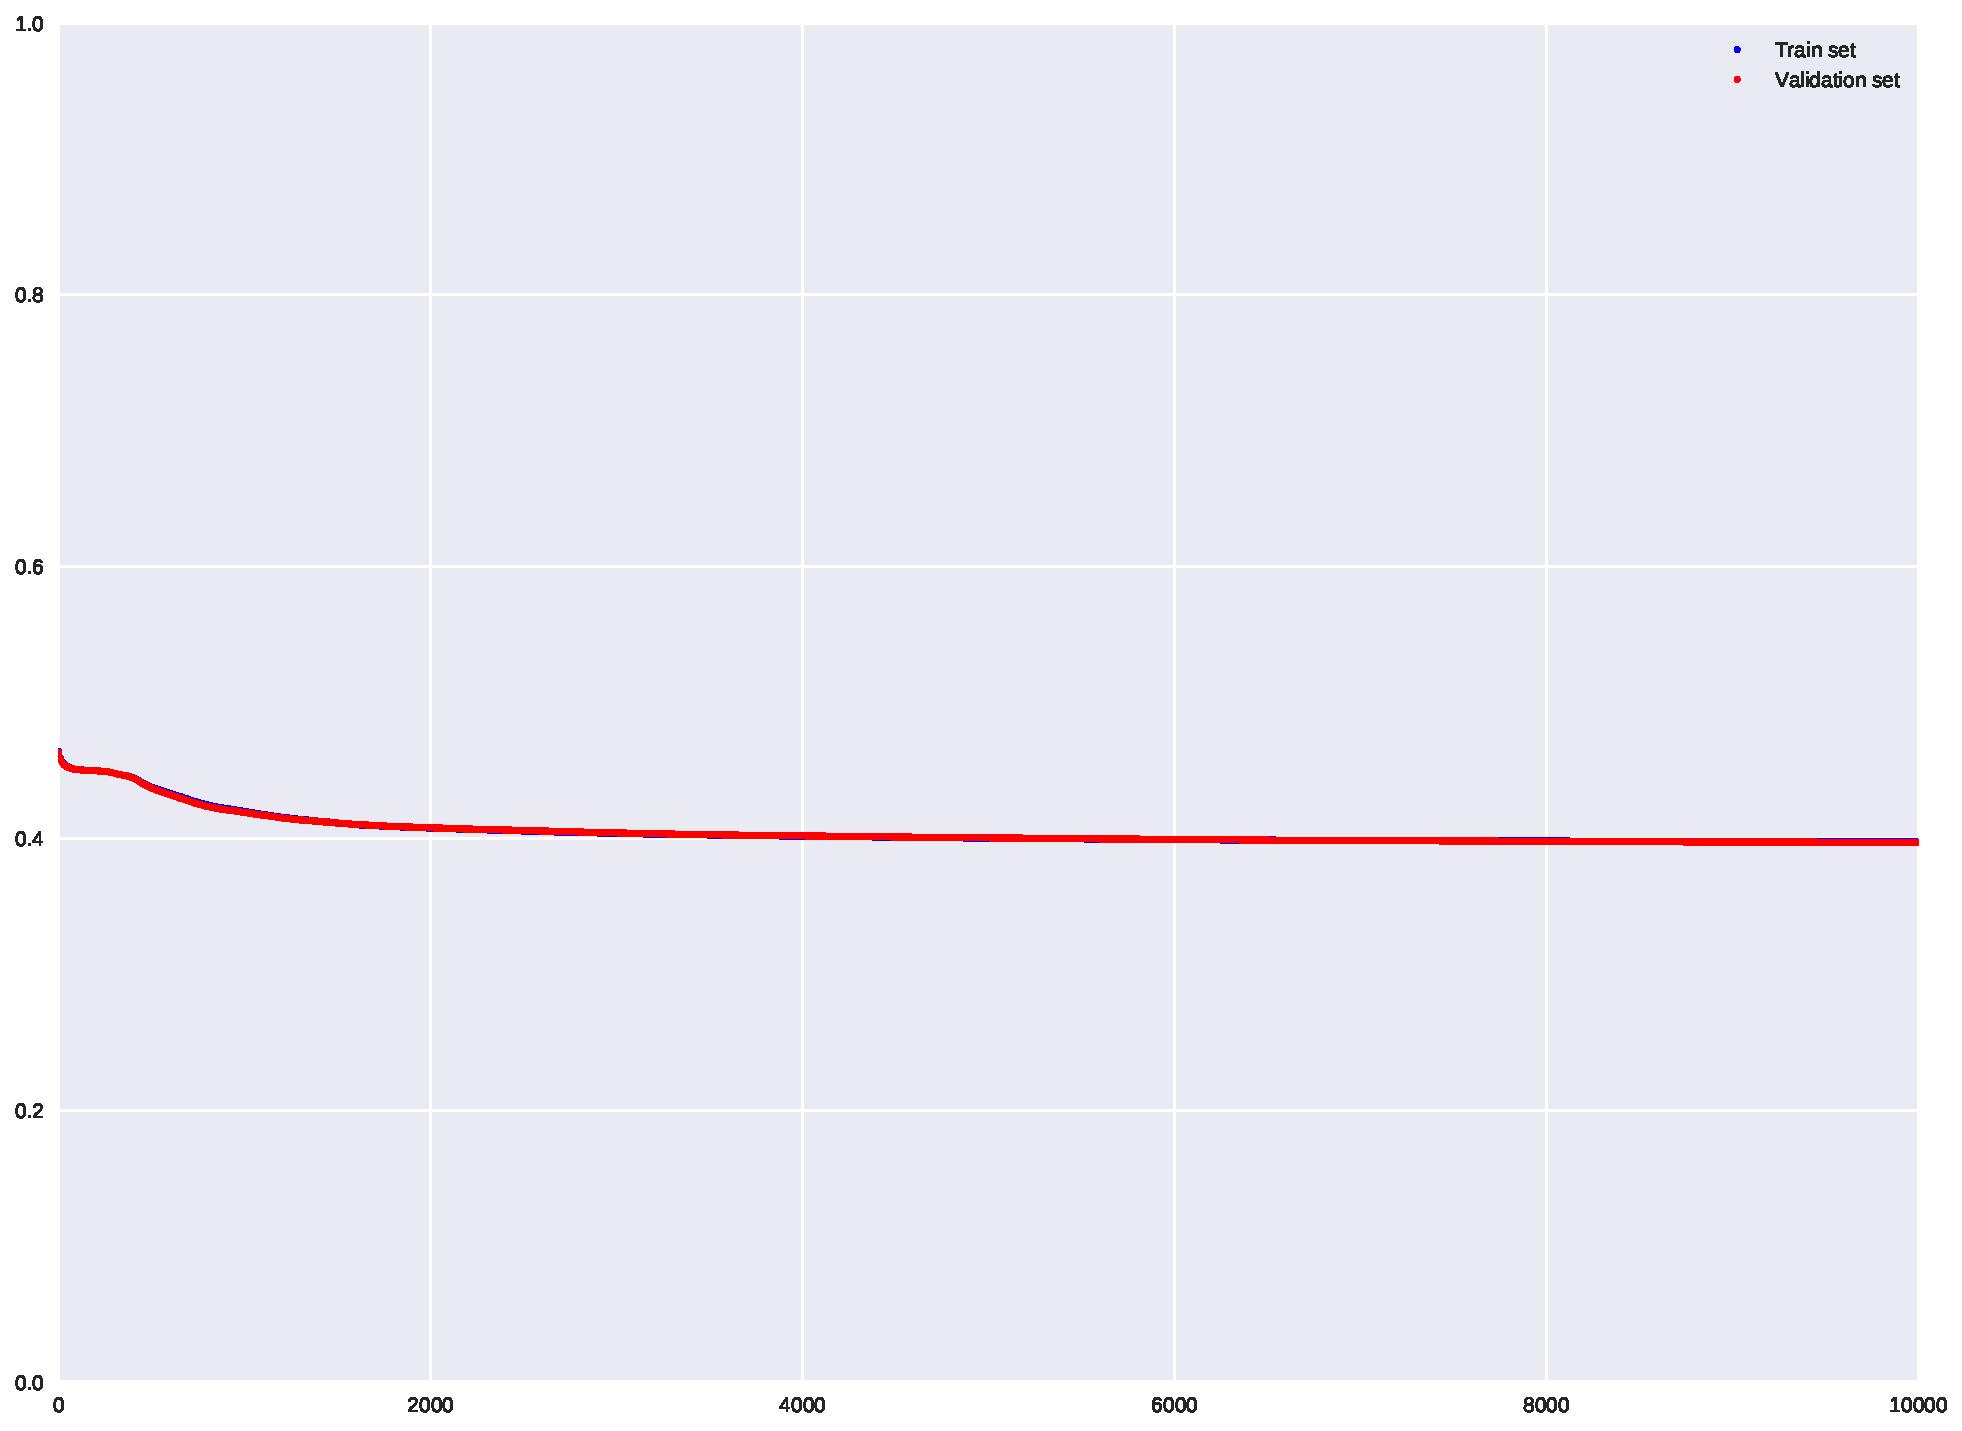
\includegraphics[width=0.9\textwidth]{learning_curves.pdf}
        \caption{Euclidean distance errors for consecutive learning epochs}
    \end{figure}
\begin{pycode}
with open('accuracy_dict.pickle', 'rb') as f:
    accuracy_dict = pickle.load(f)
print_accuracy_table(accuracy_dict)
\end{pycode}
\end{document}